\documentclass[10pt]{article}
\usepackage[margin=0.72in]{geometry}
\usepackage[T1]{fontenc}
\usepackage{graphicx}
\usepackage{amsmath}
\usepackage{amssymb}
\usepackage{array}
\setlength{\parskip}{0.45em}
\setlength{\parindent}{0pt}
\begin{document}
\begin{center}
{\Large\bfseries NCP shadow reachability: exact Lean equivalence}\par
{\small 2026-10-21; THM-COMMUTATOR-KERNEL1 Lemma 2(b); TASK-20260822-3dd086}
\end{center}

\textbf{Scope.} This proof characterizes the minimum word length needed to
represent a signed-count shadow of translation and negation letters. It uses
the same right-of-occurrence sign convention as the earlier affine-action
proof. It makes no search-cost or elliptic-curve performance claim.

\section*{Statement and construction}
For $a\in\mathbb Z^B$, write $\|a\|_1=\sum_i|a_i|$. The sign $e$ belongs to
$\{+1,-1\}$. The penalty $m(e,a)$ is $0$ for $e=+1$ with every $a_i\geq0$,
$1$ for $e=-1$, and $2$ for $e=+1$ with some $a_i<0$. Lean proves, for every
$B$, $a$, and degree bound $d$,
\[
 (\exists w,\ |w|\leq d\ \land\ \operatorname{shadow}(w)=(e,a))
 \quad\Longleftrightarrow\quad \|a\|_1+m(e,a)\leq d.
\]
The lower bound charges one letter per unit of signed-count weight and the
necessary negations. For the upper bound, $T^+$ and $T^-$ list the positive
and negative coordinate counts. The three exact constructions are
$T^+$, $T^-\nu T^+$, and $T^+\nu T^-\nu$.

\begin{center}
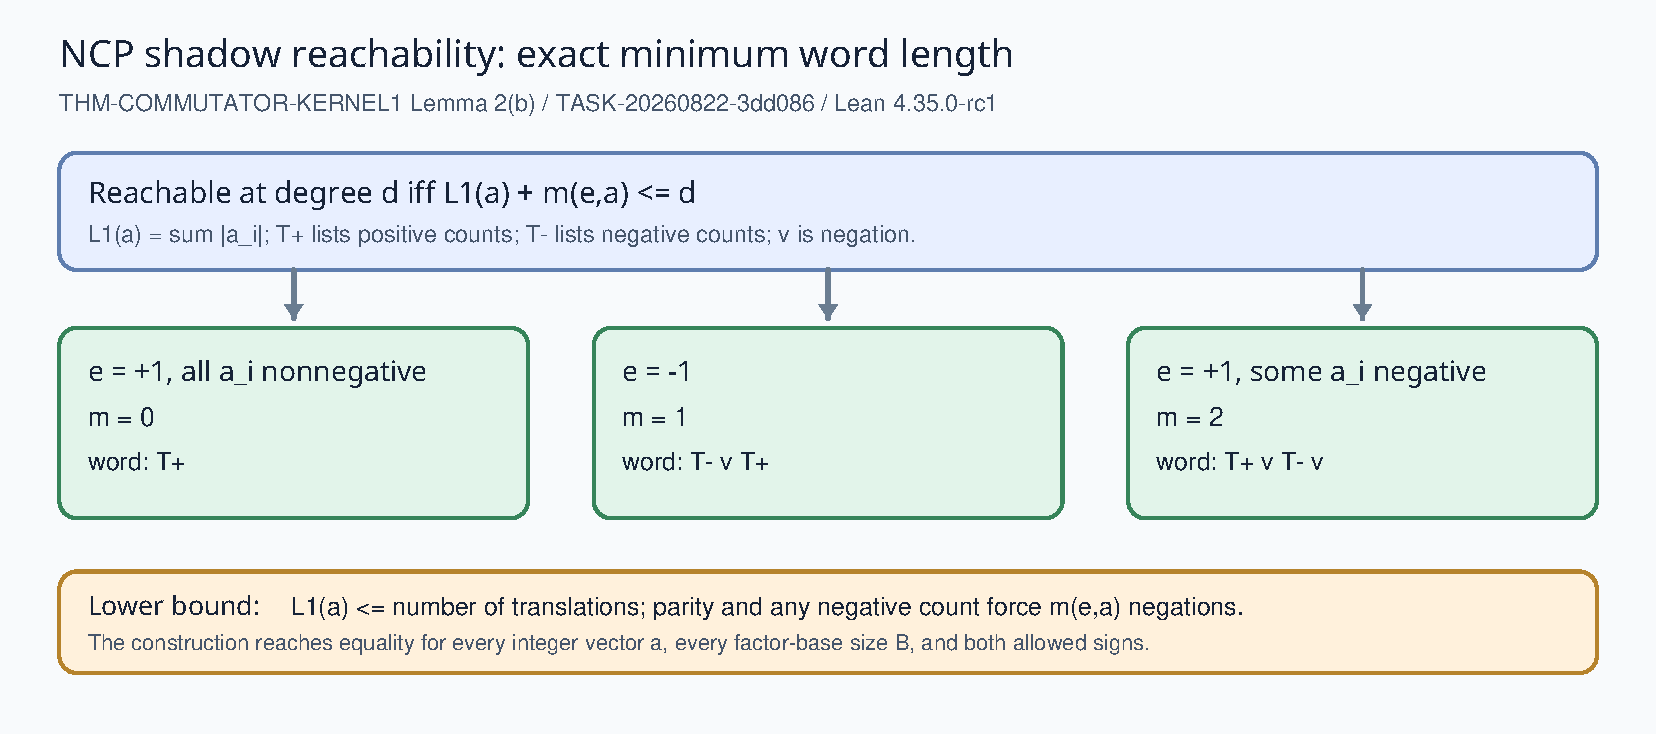
\includegraphics[width=\linewidth]{diagram.pdf}
\end{center}

\section*{Validation and limits}
\begin{tabular}{|p{0.31\linewidth}|p{0.59\linewidth}|}\hline
Check & Observed result \\ \hline
Pinned Lean target & Machine verified on Lean 4.35.0-rc1; project audit passed 498 theorem declarations using standard axioms only. Independent semantic review remains pending. \\ \hline
Direct shadow crosscheck & 28 $(B,d)$ cases, 9,190 exhaustive word evaluations, zero missing or extra shadows for $B=0..3$, $d=0..6$. \\ \hline
Complete target corpus & 65 machine verified; zero failed; zero infrastructure failures; one theorem file absent (NCP commutator-ideal refutation). \\ \hline
\end{tabular}

The bounded crosscheck compares unreduced shadow pairs. The formal theorem
holds at every size, but it does not prove the path-algebra kernel ideal,
elliptic-curve code refinement, NC search cost, or ECDLP performance. No new
timing datum was produced, so canonical numerical dashboards are unchanged.

\end{document}
